% answers.tex —— 2009 年·普通高等学校招生考试·天津卷·文科 · 参考答案与详细解析片段
% 由 tools/generate_projects.py 依来源总账自 2009/2009_数学真题_天津文_试题.md + 2009/2009_数学真题_天津文_解析正文.md + 2009/2009_数学真题_天津文_答案要点.md 生成，勿手改（改源 MD 后重跑）


\begin{gktip}
固定候选 PDF 仅含题面，无答案、解析和评分标准，原卷亦未标分值；以下为非官方编者独立推导，官方答案字段为空。题面文字层只作定位，公式、分数、根号与四幅图均以 600 dpi 原页复核。
\end{gktip}

\begin{answer}
\gksolhead{1}{}

\textbf{题目}：

$\mathrm i$ 是虚数单位，$\dfrac{5\mathrm i}{2-\mathrm i}=$（　）

（A）$1+2\mathrm i$

（B）$-1-2\mathrm i$

（C）$1-2\mathrm i$

（D）$-1+2\mathrm i$

\Needspace{4\baselineskip}
\textbf{解析}

\nopagebreak[4]
\[\frac{5\mathrm i}{2-\mathrm i}
=\frac{5\mathrm i(2+\mathrm i)}{(2-\mathrm i)(2+\mathrm i)}
=\frac{10\mathrm i+5\mathrm i^2}{5}
=\frac{-5+10\mathrm i}{5}=-1+2\mathrm i,\]

选 D。

\gkanswer{答案：D。}

\end{answer}
\begin{answer}
\gksolhead{2}{}

\textbf{题目}：

设变量 $x,y$ 满足约束条件 $\begin{cases}x+y\geqslant3,\\ x-y\geqslant-1,\\ 2x-y\leqslant3,\end{cases}$ 则目标函数 $z=2x+3y$ 的最小值为（　）

（A）$6$

（B）$7$

（C）$8$

（D）$23$

\Needspace{4\baselineskip}
\textbf{解析}

\Needspace{5\baselineskip}
作出可行域，三边两两相交得顶点 $(1,2)$、$(2,1)$、$(4,5)$。目标值

\nopagebreak[4]
\[z(1,2)=2+6=8,\qquad z(2,1)=4+3=7,\qquad z(4,5)=8+15=23 .\]

最小值为 $7$，选 B。

\gkanswer{答案：B。}

\end{answer}
\begin{answer}
\gksolhead{3}{}

\textbf{题目}：

设 $x\in\mathbf R$，则「$x=1$」是「$x^3=x$」的（　）

（A）充分而不必要条件

（B）必要而不充分条件

（C）充要条件

（D）既不充分也不必要条件

\Needspace{4\baselineskip}
\textbf{解析}

$x=1$ 时 $x^3=1=x$，故充分。

反之 $x^3=x\iff x(x-1)(x+1)=0\iff x=0,\pm1$，不一定是 $1$，故不必要。

所以是充分而不必要条件，选 A。

\gkanswer{答案：A。}

\end{answer}
\begin{answer}
\gksolhead{4}{}

\textbf{题目}：

设双曲线 $\dfrac{x^2}{a^2}-\dfrac{y^2}{b^2}=1$（$a>0$，$b>0$）的虚轴长为 $2$，焦距为 $2\sqrt3$，则双曲线的渐近线方程为（　）

（A）$y=\pm\sqrt2x$

（B）$y=\pm2x$

（C）$y=\pm\dfrac{\sqrt2}{2}x$

（D）$y=\pm\dfrac12x$

\Needspace{4\baselineskip}
\textbf{解析}

\Needspace{5\baselineskip}
虚轴长 $2b=2$，故 $b=1$；焦距 $2c=2\sqrt3$，故 $c=\sqrt3$。于是

\nopagebreak[4]
\[a^2=c^2-b^2=3-1=2 .\]

\Needspace{5\baselineskip}
渐近线为

\nopagebreak[4]
\[y=\pm\frac ba x=\pm\frac{1}{\sqrt2}x=\pm\frac{\sqrt2}{2}x,\]

选 C。

\gkanswer{答案：C。}

\end{answer}
\begin{answer}
\gksolhead{5}{}

\textbf{题目}：

设 $a=\log_{\frac13}2$，$b=\log_{\frac12}\dfrac13$，$c=\left(\dfrac12\right)^{0.3}$，则（　）

（A）$a<b<c$

（B）$a<c<b$

（C）$b<c<a$

（D）$b<a<c$

\Needspace{4\baselineskip}
\textbf{解析}

\nopagebreak[4]
\[a=\log_{\frac13}2=-\log_3 2<0,\]

\nopagebreak[4]
\[b=\log_{\frac12}\frac13=\log_2 3>1,\]

\nopagebreak[4]
\[c=\left(\frac12\right)^{0.3}=2^{-0.3}\in(0,1).\]

故 $a<c<b$，选 B。

\gkanswer{答案：B。}

\end{answer}
\begin{answer}
\gksolhead{6}{}

\textbf{题目}：

阅读如图的程序框图，则输出的 $S=$（　）
\nopagebreak[4]
\begin{center}% 2009 年天津卷文科第 6 题：求 S=1²+2²+3²+4² 的程序框图。
% 来源 PDF：普通高考/2009/2009天津文.pdf，SHA256 5d3e0110cc9145311eed3af1cf0f691ee327cbcba3a0d245e88d635fc136203f
% 原页：第 1 页（A3 三栏）第 1 栏下部，印刷页 563。
% 重绘依据：开始 → S=0,i=1 → S=S+i² → i=i+1 → 判断 i>4；否（左）回到 S=S+i²，
%   是（下）→ 输出 S → 结束；箭头与原图方向一致。
\begin{tikzpicture}[scale=0.9, semithick, >=Stealth,
  node distance=5mm, every node/.style={inner sep=3pt, font=\small}]
  \node (start) [draw, rounded corners=4pt, minimum width=2.0cm, minimum height=0.65cm] {开始};
  \node (init) [draw, minimum width=3.4cm, minimum height=0.65cm, below=of start] {$S=0,\ i=1$};
  \node (add) [draw, minimum width=3.4cm, minimum height=0.65cm, below=of init] {$S=S+i^2$};
  \node (inc) [draw, minimum width=3.4cm, minimum height=0.65cm, below=of add] {$i=i+1$};
  \node (cond) [draw, diamond, aspect=2.0, minimum width=3.2cm, minimum height=1.0cm, below=of inc] {$i>4$};
  \node (out) [draw, trapezium, trapezium left angle=70, trapezium right angle=110,
    minimum width=3.0cm, minimum height=0.65cm, below=of cond] {输出 $S$};
  \node (end) [draw, rounded corners=4pt, minimum width=2.0cm, minimum height=0.65cm, below=of out] {结束};
  \draw[->] (start) -- (init);
  \draw[->] (init) -- (add);
  \draw[->] (add) -- (inc);
  \draw[->] (inc) -- (cond);
  \draw[->] (cond) -- (out);
  \node[anchor=west] at ($(cond.south)!0.5!(out.north)+(14pt,-4pt)$) {是};
  \draw[->] (cond.east) -- ++(1.1,0) |- node[pos=0.25, right] {否} (add.east);
  \draw[->] (out) -- (end);
\end{tikzpicture}
\end{center}
\nopagebreak[4]
（A）$14$

（B）$20$

（C）$30$

（D）$55$

\Needspace{4\baselineskip}
\textbf{解析}

\Needspace{5\baselineskip}
循环变量依次取 $i=1,2,3,4$，每次执行 $S\leftarrow S+i^2$，当 $i>4$ 时输出。故

\nopagebreak[4]
\[S=1^2+2^2+3^2+4^2=1+4+9+16=30,\]

选 C。

\gkanswer{答案：C。}

\end{answer}
\begin{answer}
\gksolhead{7}{}

\textbf{题目}：

已知函数 $f(x)=\sin\left(\omega x+\dfrac{\pi}{4}\right)$（$x\in\mathbf R$，$\omega>0$）的最小正周期为 $\pi$．将 $y=f(x)$ 的图象向左平移 $|\varphi|$ 个单位长度，所得图象关于 $y$ 轴对称，则 $\varphi$ 的一个值是（　）

（A）$\dfrac{\pi}{2}$

（B）$\dfrac{3\pi}{8}$

（C）$\dfrac{\pi}{4}$

（D）$\dfrac{\pi}{8}$

\Needspace{4\baselineskip}
\textbf{解析}

\Needspace{5\baselineskip}
由最小正周期

\nopagebreak[4]
\[T=\frac{2\pi}{\omega}=\pi\ \Longrightarrow\ \omega=2 .\]

\Needspace{5\baselineskip}
左移 $|\varphi|$ 后

\nopagebreak[4]
\[y=\sin\left(2(x+|\varphi|)+\frac\pi4\right)
=\sin\left(2x+2|\varphi|+\frac\pi4\right).\]

\Needspace{5\baselineskip}
所得图象关于 $y$ 轴对称，需为偶函数，即

\nopagebreak[4]
\[2|\varphi|+\frac\pi4=\frac\pi2+k\pi
\ \Longrightarrow\ |\varphi|=\frac\pi8+\frac{k\pi}{2}\quad(k\in\mathbf Z).\]

取 $k=0$ 得 $|\varphi|=\dfrac\pi8$，故 $\varphi=\pm\dfrac\pi8$。选项中只有 $\dfrac\pi8$，选 D。

\gkanswer{答案：D。}

\end{answer}
\begin{answer}
\gksolhead{8}{}

\textbf{题目}：

设函数 $f(x)=\begin{cases}x^2-4x+6,&x\geqslant0,\\ x+6,&x<0,\end{cases}$ 则不等式 $f(x)>f(1)$ 的解集是（　）

（A）$(-3,1)\cup(3,+\infty)$

（B）$(-3,1)\cup(2,+\infty)$

（C）$(-1,1)\cup(3,+\infty)$

（D）$(-\infty,-3)\cup(1,3)$

\Needspace{4\baselineskip}
\textbf{解析}

$f(1)=1-4+6=3$。

\Needspace{5\baselineskip}
$x\geqslant0$ 时：

\nopagebreak[4]
\[x^2-4x+6>3\iff x^2-4x+3>0\iff x<1\ \text{\text{或}}\ x>3,\]

结合 $x\geqslant0$ 得 $[0,1)\cup(3,+\infty)$。

\Needspace{5\baselineskip}
$x<0$ 时：

\nopagebreak[4]
\[x+6>3\iff x>-3,\]

得 $(-3,0)$。

\Needspace{5\baselineskip}
合并得

\nopagebreak[4]
\[(-3,1)\cup(3,+\infty),\]

选 A。

\gkanswer{答案：A。}

\end{answer}
\begin{answer}
\gksolhead{9}{}

\textbf{题目}：

设 $x,y\in\mathbf R$，$a>1$，$b>1$．若 $a^x=b^y=3$，$a+b=2\sqrt3$，则 $\dfrac1x+\dfrac1y$ 的最大值为（　）

（A）$2$

（B）$\dfrac32$

（C）$1$

（D）$\dfrac12$

\Needspace{4\baselineskip}
\textbf{解析}

\Needspace{5\baselineskip}
由 $a^x=3$ 得 $x=\log_a 3$，故

\nopagebreak[4]
\[\frac1x=\log_3 a .\]

\Needspace{5\baselineskip}
同理 $\dfrac1y=\log_3 b$。于是

\nopagebreak[4]
\[\frac1x+\frac1y=\log_3(ab)
\leqslant\log_3\left(\frac{a+b}{2}\right)^2
=\log_3\left(\sqrt3\right)^2=\log_3 3=1,\]

等号在 $a=b=\sqrt3$ 时成立。最大值为 $1$，选 C。

\gkanswer{答案：C。}

\end{answer}
\begin{answer}
\gksolhead{10}{}

\textbf{题目}：

设函数 $f(x)$ 在 $\mathbf R$ 上的导函数为 $f'(x)$，且 $2f(x)+xf'(x)>x^2$．下面的不等式在 $\mathbf R$ 内恒成立的是（　）

（A）$f(x)>0$

（B）$f(x)<0$

（C）$f(x)>x$

（D）$f(x)<x$

\Needspace{4\baselineskip}
\textbf{解析}

\Needspace{5\baselineskip}
令

\nopagebreak[4]
\[g(x)=x^2f(x)-\frac{x^4}{4},\]

\Needspace{5\baselineskip}
则

\nopagebreak[4]
\[g'(x)=2xf(x)+x^2f'(x)-x^3
=x\left[2f(x)+xf'(x)-x^2\right].\]

\Needspace{5\baselineskip}
由题设方括号为正：$x>0$ 时 $g'(x)>0$，$x<0$ 时 $g'(x)<0$。故 $g$ 在 $x=0$ 取最小值

\nopagebreak[4]
\[g(0)=0 .\]

\Needspace{5\baselineskip}
于是 $x\ne0$ 时

\nopagebreak[4]
\[x^2f(x)>\frac{x^4}{4}\ \Longrightarrow\ f(x)>\frac{x^2}{4}>0 .\]

又 $f(0)$ 处不等式给出 $2f(0)>0$，故 $f(x)>0$ 在 $\mathbf R$ 上恒成立，选 A。

\gkanswer{答案：A。}

\end{answer}
\begin{answer}
\gksolhead{11}{}

\textbf{题目}：

如图，$AA_1$ 与 $BB_1$ 相交于点 $O$，$AB\parallel A_1B_1$ 且 $AB=\dfrac12A_1B_1$，若 $\triangle AOB$ 的外接圆直径为 $1$，则 $\triangle A_1OB_1$ 的外接圆直径为\gkblank{}．
\nopagebreak[4]
\begin{center}% 2009 年天津卷文科第 11 题：AA_1 与 BB_1 相交于 O，AB∥A_1B_1 且 AB=½A_1B_1。
% 来源 PDF：普通高考/2009/2009天津文.pdf，SHA256 5d3e0110cc9145311eed3af1cf0f691ee327cbcba3a0d245e88d635fc136203f
% 原页：第 1 页（A3 三栏）第 2 栏中部，印刷页 563。
% 重绘依据：AB 与 A_1B_1 为两条平行线段，按原图呈「X」形交叉（A 连 A_1、B 连 B_1），
%   O 为交点；AB 较短、A_1B_1 较长，长度比 1:2。
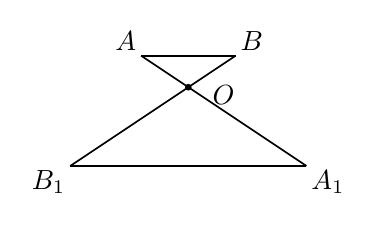
\begin{tikzpicture}[scale=1.0, semithick, every node/.style={inner sep=1.5pt}]
  \coordinate (A)  at (0.9,1.4);
  \coordinate (B)  at (2.1,1.4);
  \coordinate (B1) at (0,0);
  \coordinate (A1) at (3.0,0);
  \coordinate (O)  at (1.5,1.0);
  \draw (A) -- (B);
  \draw (A1) -- (B1);
  \draw (A) -- (A1);
  \draw (B) -- (B1);
  \fill (O) circle (1.2pt);
  \node[anchor=south east] at (A) {$A$};
  \node[anchor=south west] at (B) {$B$};
  \node[anchor=north east] at (B1) {$B_1$};
  \node[anchor=north west] at (A1) {$A_1$};
  \node[anchor=west] at ([xshift=7pt,yshift=-3pt]O) {$O$};
\end{tikzpicture}
\end{center}
\nopagebreak[4]
\Needspace{4\baselineskip}
\textbf{解析}

\Needspace{5\baselineskip}
由 $AB\parallel A_1B_1$ 得

\nopagebreak[4]
\[\triangle AOB\sim\triangle A_1OB_1,\]

\Needspace{5\baselineskip}
相似比为

\nopagebreak[4]
\[\frac{A_1B_1}{AB}=2 .\]

\Needspace{5\baselineskip}
相似三角形外接圆直径之比等于相似比，故 $\triangle A_1OB_1$ 的外接圆直径为

\nopagebreak[4]
\[2\times1=2 .\]

\gkanswer{答案：$2$。}

\end{answer}
\begin{answer}
\gksolhead{12}{}

\textbf{题目}：

如图是一个几何体的三视图，若它的体积是 $3\sqrt3$，则 $a=$\gkblank{}．
\nopagebreak[4]
\begin{center}% 2009 年天津卷文科第 12 题：直三棱柱的三视图。
% 来源 PDF：普通高考/2009/2009天津文.pdf，SHA256 5d3e0110cc9145311eed3af1cf0f691ee327cbcba3a0d245e88d635fc136203f
% 原页：第 1 页（A3 三栏）第 2 栏中部，印刷页 563。
% 重绘依据：正视图为 3×a 矩形；侧视图为底边 2、高 a 的三角形；俯视图为 3×2 矩形，
%   中间一条平行于长的实线把深度分成 1 与 1 两段；尺寸与标注按原图。
\begin{tikzpicture}[scale=0.95, semithick, every node/.style={inner sep=1.2pt}]
  % 正视图
  \draw (0,1.5) rectangle (3,3.0);
  \node[anchor=east] at (-0.1,2.25) {$a$};
  \node[anchor=north] at (1.5,1.35) {正视图};
  % 侧视图
  \draw (4.2,1.5) -- (5.8,1.5) -- (5.0,3.0) -- cycle;
  \node[anchor=north] at (5.0,1.05) {侧视图};
  \node[anchor=north] at (5.0,1.32) {$2$};
  % 俯视图
  \draw (0,0) rectangle (3,1.0);
  \draw (0,0.5) -- (3,0.5);
  \node[anchor=north] at (1.5,-0.15) {俯视图};
  \node[anchor=east] at (-0.1,0.25) {$1$};
  \node[anchor=east] at (-0.1,0.75) {$1$};
\end{tikzpicture}
\end{center}
\nopagebreak[4]
\Needspace{4\baselineskip}
\textbf{解析}

\Needspace{5\baselineskip}
由三视图，该几何体是底面为直角三角形、高为 $a$ 的直三棱柱：底面两直角边分别为 $3$ 与 $2$。

\nopagebreak[4]
\[V=\frac12\cdot3\cdot2\cdot a=3a .\]

\Needspace{5\baselineskip}
由 $V=3\sqrt3$ 得

\nopagebreak[4]
\[a=\sqrt3 .\]

\gkanswer{答案：$\sqrt3$。}

\end{answer}
\begin{answer}
\gksolhead{13}{}

\textbf{题目}：

设全集 $U=A\cup B=\{x\in\mathbf N^*\mid \lg x<1\}$，若 $A\cap(\complement_UB)=\{m\mid m=2n+1,\ n=0,1,2,3,4\}$，则集合 $B=$\gkblank{}．

\Needspace{4\baselineskip}
\textbf{解析}

\nopagebreak[4]
\[\lg x<1\iff 0<x<10,\]

\Needspace{5\baselineskip}
故

\nopagebreak[4]
\[U=\{1,2,3,4,5,6,7,8,9\} .\]

\Needspace{5\baselineskip}
又

\nopagebreak[4]
\[A\cap(\complement_UB)=A\setminus B=\{1,3,5,7,9\},\]

\Needspace{5\baselineskip}
即 $U$ 中的奇数全在 $A\setminus B$ 中（不在 $B$），偶数全在 $B$ 中。故

\nopagebreak[4]
\[B=\{2,4,6,8\} .\]

\gkanswer{答案：$\{2,4,6,8\}$。}

\end{answer}
\begin{answer}
\gksolhead{14}{}

\textbf{题目}：

若圆 $x^2+y^2=4$ 与圆 $x^2+y^2+2ay-6=0$（$a>0$）的公共弦的长为 $2\sqrt3$，则 $a=$\gkblank{}．

\Needspace{4\baselineskip}
\textbf{解析}

\Needspace{5\baselineskip}
两圆方程相减：

\nopagebreak[4]
\[(x^2+y^2+2ay-6)-(x^2+y^2)= -4
\ \Longrightarrow\ 2ay=2\ \Longrightarrow\ y=\frac1a .\]

\Needspace{5\baselineskip}
圆 $x^2+y^2=4$ 被该直线截得的半弦长为

\nopagebreak[4]
\[\sqrt{4-\frac1{a^2}} .\]

\Needspace{5\baselineskip}
由弦长 $2\sqrt3$：

\nopagebreak[4]
\[\sqrt{4-\frac1{a^2}}=\sqrt3
\ \Longrightarrow\ \frac1{a^2}=1
\ \Longrightarrow\ a=1\ (a>0).\]

\gkanswer{答案：$1$。}

\end{answer}
\begin{answer}
\gksolhead{15}{}

\textbf{题目}：

若等边 $\triangle ABC$ 的边长为 $2\sqrt3$，平面内一点 $M$ 满足 $\overrightarrow{CM}=\dfrac16\overrightarrow{CB}+\dfrac23\overrightarrow{CA}$，则 $\overrightarrow{MA}\cdot\overrightarrow{MB}=$\gkblank{}．

\Needspace{4\baselineskip}
\textbf{解析}

\Needspace{5\baselineskip}
取 $C$ 为原点，记 $\boldsymbol a=\overrightarrow{CA}$、$\boldsymbol b=\overrightarrow{CB}$。等边三角形边长 $2\sqrt3$：

\nopagebreak[4]
\[|\boldsymbol a|=|\boldsymbol b|=2\sqrt3,\qquad
\boldsymbol a\cdot\boldsymbol b=12\cos60^\circ=6 .\]

\Needspace{5\baselineskip}
由

\nopagebreak[4]
\[\overrightarrow{CM}=\frac16\boldsymbol b+\frac23\boldsymbol a,\]

\Needspace{5\baselineskip}
得

\nopagebreak[4]
\[\overrightarrow{MA}=\boldsymbol a-\overrightarrow{CM}=\frac13\boldsymbol a-\frac16\boldsymbol b,\]

\nopagebreak[4]
\[\overrightarrow{MB}=\boldsymbol b-\overrightarrow{CM}=-\frac23\boldsymbol a+\frac56\boldsymbol b .\]

\Needspace{5\baselineskip}
于是

\nopagebreak[4]
\[\overrightarrow{MA}\cdot\overrightarrow{MB}
=-\frac29|\boldsymbol a|^2+\frac7{18}\boldsymbol a\cdot\boldsymbol b-\frac5{36}|\boldsymbol b|^2
=-\frac83+\frac73-\frac53=-2 .\]

\gkanswer{答案：$-2$。}

\end{answer}
\begin{answer}
\gksolhead{16}{}

\textbf{题目}：

若关于 $x$ 的不等式 $(2x-1)^2<ax^2$ 的解集中的整数恰好有 $3$ 个，则实数 $a$ 的取值范围是\gkblank{}．

\Needspace{4\baselineskip}
\textbf{解析}

\Needspace{5\baselineskip}
不等式即

\nopagebreak[4]
\[(4-a)x^2-4x+1<0 .\]

按 $a$ 的取值分类。

\begin{itemize}
\item $a\leqslant0$：左端 $(2x-1)^2\geqslant0$，右端 $ax^2\leqslant0$，严格小于不可能成立，无解。
\item $a=4$：$-4x+1<0\iff x>\dfrac14$，无穷多整数解。
\item $a>4$：二次项系数 $4-a<0$，抛物线开口向下，$g(x)<0$ 在两根之外，解集为两条无界射线，含无穷多整数，不合。
\item $0<a<4$：开口向上，$g<0$ 在两根之间。方程
\end{itemize}

\nopagebreak[4]
\[(4-a)x^2-4x+1=0\]

\Needspace{5\baselineskip}
的两根为

\nopagebreak[4]
\[\frac{4\pm\sqrt{16-4(4-a)}}{2(4-a)}
=\frac{2\pm\sqrt a}{4-a},\]

\Needspace{5\baselineskip}
即

\nopagebreak[4]
\[r_1=\frac{2-\sqrt a}{4-a}=\frac1{2+\sqrt a},\qquad
r_2=\frac{2+\sqrt a}{4-a}=\frac1{2-\sqrt a}.\]

因 $0<a<4$，有 $0<r_1<\dfrac12<r_2$，故解集为 $(r_1,r_2)$，其中的整数从 $1$ 开始。

\Needspace{5\baselineskip}
恰有 $3$ 个整数，只能是 $1,2,3$，故需

\nopagebreak[4]
\[r_1<1\ (\text{\text{自动成立}}),\qquad 3<r_2\leqslant4 .\]

\nopagebreak[4]
\[\frac1{2-\sqrt a}>3
\iff 2-\sqrt a<\frac13
\iff \sqrt a>\frac53
\iff a>\frac{25}{9},\]

\nopagebreak[4]
\[\frac1{2-\sqrt a}\leqslant4
\iff 2-\sqrt a\geqslant\frac14
\iff \sqrt a\leqslant\frac74
\iff a\leqslant\frac{49}{16}.\]

\Needspace{5\baselineskip}
故

\nopagebreak[4]
\[a\in\left(\frac{25}{9},\frac{49}{16}\right].\]

端点核对：$a=\dfrac{25}{9}$ 时 $r_2=3$，区间 $\left(\dfrac3{11},3\right)$ 内只有 $1,2$，不合；$a=\dfrac{49}{16}$ 时 $r_2=4$，区间 $\left(\frac4{15},4\right)$ 内为 $1,2,3$，符合。

\gkanswer{答案：$\left(\dfrac{25}{9},\dfrac{49}{16}\right]$。}

\end{answer}
\begin{answer}
\gksolhead{17}{}

\textbf{题目}：

在 $\triangle ABC$ 中，$BC=\sqrt5$，$AC=3$，$\sin C=2\sin A$．

（1）求 $AB$ 的值；

（2）求 $\sin\left(2A-\dfrac{\pi}{4}\right)$ 的值．

\Needspace{4\baselineskip}
\textbf{解析}

\Needspace{5\baselineskip}
（1）由正弦定理

\nopagebreak[4]
\[\frac{AB}{\sin C}=\frac{BC}{\sin A},\]

\Needspace{5\baselineskip}
故

\nopagebreak[4]
\[AB=BC\cdot\frac{\sin C}{\sin A}=BC\cdot2=2\sqrt5 .\]

\Needspace{5\baselineskip}
（2）由余弦定理

\nopagebreak[4]
\[\cos A=\frac{AB^2+AC^2-BC^2}{2\cdot AB\cdot AC}
=\frac{20+9-5}{12\sqrt5}=\frac{24}{12\sqrt5}=\frac{2}{\sqrt5},\]

\Needspace{5\baselineskip}
故 $\sin A=\dfrac1{\sqrt5}$。于是

\nopagebreak[4]
\[\sin2A=2\sin A\cos A=\frac45,\]

\nopagebreak[4]
\[\cos2A=\cos^2A-\sin^2A=\frac45-\frac15=\frac35 .\]

\nopagebreak[4]
\[\sin\left(2A-\frac\pi4\right)
=\sin2A\cos\frac\pi4-\cos2A\sin\frac\pi4
=\frac{4/5-3/5}{\sqrt2}=\frac{\sqrt2}{10} .\]

\gkanswer{答案：（1）$AB=2\sqrt5$；（2）$\dfrac{\sqrt2}{10}$。}

\end{answer}
\begin{answer}
\gksolhead{18}{}

\textbf{题目}：

为了了解某工厂开展群众体育活动的情况，拟采用分层抽样的方法从 $A,B,C$ 三个区中抽取 $7$ 个工厂进行调查，已知 $A,B,C$ 区中分别有 $18$，$27$，$18$ 个工厂．

（1）求从 $A,B,C$ 区中分别抽取的工厂个数；

（2）若从抽取的 $7$ 个工厂中随机抽取 $2$ 个进行调查结果的对比，用列举法计算这 $2$ 个工厂中至少有 $1$ 个来自 $A$ 区的概率．

\Needspace{4\baselineskip}
\textbf{解析}

\Needspace{5\baselineskip}
（1）三个区共有

\nopagebreak[4]
\[18+27+18=63\]

\Needspace{5\baselineskip}
个工厂，样本量 $7$，抽样比为 $\dfrac19$。故各区分得

\nopagebreak[4]
\[18\times\frac19=2,\qquad 27\times\frac19=3,\qquad 18\times\frac19=2 .\]

\Needspace{5\baselineskip}
（2）$7$ 个工厂中来自 $A$ 区的有 $2$ 个。任取 $2$ 个的取法共

\nopagebreak[4]
\[\mathrm C_7^2=21,\]

\Needspace{5\baselineskip}
两个都不来自 $A$ 区的取法为

\nopagebreak[4]
\[\mathrm C_5^2=10 .\]

\Needspace{5\baselineskip}
故至少一个来自 $A$ 区的概率

\nopagebreak[4]
\[P=1-\frac{10}{21}=\frac{11}{21} .\]

\gkanswer{答案：（1）$2,3,2$；（2）$\dfrac{11}{21}$。}

\end{answer}
\begin{answer}
\gksolhead{19}{}

\textbf{题目}：

如图，在四棱锥 $P-ABCD$ 中，$PD\perp$ 平面 $ABCD$，$AD\perp CD$，且 $DB$ 平分 $\angle ADC$，$E$ 为 $PC$ 的中点，$AD=CD=1$，$DB=2\sqrt2$．
\nopagebreak[4]
\begin{center}% 2009 年天津卷文科第 19 题：四棱锥 P-ABCD，PD⊥平面 ABCD，E 为 PC 中点。
% 来源 PDF：普通高考/2009/2009天津文.pdf，SHA256 5d3e0110cc9145311eed3af1cf0f691ee327cbcba3a0d245e88d635fc136203f
% 原页：第 2 页（A3 三栏）第 1 栏，印刷页 564。
% 重绘依据：按原图 P 在 D 上方，D 左下、C 右下、B 最右、A 在 D 上方偏左；
%   棱 PA、PB、PC 实线，底面边 AB、BC、CD、DA 与对角线 DB 实线，AC 画虚线；
%   E 为 PC 中点并标出。
\begin{tikzpicture}[scale=1.0, semithick, every node/.style={inner sep=1.2pt}]
  \coordinate (P) at (0.5,3.6);
  \coordinate (D) at (0,0);
  \coordinate (C) at (2.4,-0.3);
  \coordinate (B) at (4.2,1.3);
  \coordinate (A) at (0.9,1.6);
  \coordinate (E) at ($(P)!0.5!(C)$);
  % 底面
  \draw (A) -- (B) -- (C) -- (D) -- cycle;
  \draw (D) -- (B);
  \draw[dashed] (A) -- (C);
  % 侧棱
  \draw (P) -- (A);
  \draw (P) -- (B);
  \draw (P) -- (C);
  % E
  \fill (E) circle (1.2pt);
  \node[anchor=south] at (P) {$P$};
  \node[anchor=north east] at (D) {$D$};
  \node[anchor=north west] at (C) {$C$};
  \node[anchor=west] at (B) {$B$};
  \node[anchor=east] at (A) {$A$};
  \node[anchor=west] at ([xshift=3pt]E) {$E$};
\end{tikzpicture}
\end{center}
\nopagebreak[4]
（1）证明：$PA\parallel$ 平面 $BDE$；

（2）证明：$AC\perp$ 平面 $PBD$；

（3）求直线 $BC$ 与平面 $PBD$ 所成的角的正切值．

\Needspace{4\baselineskip}
\textbf{解析}

\Needspace{5\baselineskip}
以 $D$ 为原点，$DB$ 为 $x$ 轴，平面 $ABCD$ 为 $xy$ 平面。由 $DB$ 平分 $\angle ADC$、$AD=CD=1$、$AD\perp CD$ 得

\nopagebreak[4]
\[A\left(\frac{\sqrt2}{2},\frac{\sqrt2}{2},0\right),\quad
C\left(\frac{\sqrt2}{2},-\frac{\sqrt2}{2},0\right),\quad
B(2\sqrt2,0,0).\]

$PD\perp$ 平面，设 $P(0,0,h)$，$E$ 为 $PC$ 中点。

\Needspace{5\baselineskip}
（1）$AC$ 的中点为

\nopagebreak[4]
\[F\left(\frac{\sqrt2}{2},0,0\right),\]

\Needspace{5\baselineskip}
且 $F$ 在 $DB$ 上。在 $\triangle PAC$ 中，$E$、$F$ 分别为 $PC$、$AC$ 的中点，故

\nopagebreak[4]
\[EF\parallel PA .\]

\Needspace{5\baselineskip}
又 $EF\subset$ 平面 $BDE$，$PA\not\subset$ 平面 $BDE$，所以

\nopagebreak[4]
\[PA\parallel\text{\text{平面} }BDE .\]

\Needspace{5\baselineskip}
（2）$\overrightarrow{AC}=(0,-\sqrt2,0)$，而

\nopagebreak[4]
\[\overrightarrow{DB}=(2\sqrt2,0,0),\qquad \overrightarrow{PD}=(0,0,-h),\]

\Needspace{5\baselineskip}
故

\nopagebreak[4]
\[\overrightarrow{AC}\cdot\overrightarrow{DB}=0,\qquad
\overrightarrow{AC}\cdot\overrightarrow{PD}=0 .\]

\Needspace{5\baselineskip}
即 $AC\perp DB$、$AC\perp PD$。$DB$ 与 $PD$ 是平面 $PBD$ 内的相交直线，故

\nopagebreak[4]
\[AC\perp\text{\text{平面} }PBD .\]

\Needspace{5\baselineskip}
（3）平面 $PBD$ 即 $xz$ 平面，法向量 $\mathbf n=(0,1,0)$。

\nopagebreak[4]
\[\overrightarrow{BC}=\left(-\frac{3\sqrt2}{2},-\frac{\sqrt2}{2},0\right),\]

\nopagebreak[4]
\[|\overrightarrow{BC}|=\sqrt{\frac{18}{4}+\frac{2}{4}}=\sqrt5 .\]

\Needspace{5\baselineskip}
设 $BC$ 与平面 $PBD$ 所成角为 $\theta$：

\nopagebreak[4]
\[\sin\theta=\frac{|\overrightarrow{BC}\cdot\mathbf n|}{|\overrightarrow{BC}|}
=\frac{\sqrt2/2}{\sqrt5}=\frac{1}{\sqrt{10}} .\]

\Needspace{5\baselineskip}
故

\nopagebreak[4]
\[\tan\theta=\frac{1/\sqrt{10}}{\sqrt{1-1/10}}=\frac{1/\sqrt{10}}{3/\sqrt{10}}=\frac13 .\]

\gkanswer{答案：（1）（2）证明见解析；（3）$\dfrac13$。}

\end{answer}
\begin{answer}
\gksolhead{20}{}

\textbf{题目}：

已知等差数列 $\{a_n\}$ 的公差 $d$ 不为 $0$，设 $S_n=a_1+a_2q+\cdots+a_nq^{n-1}$，$T_n=a_1-a_2q+\cdots+(-1)^{n-1}a_nq^{n-1}$，$q\neq0$，$n\in\mathbf N^*$．

（1）若 $q=1$，$a_1=1$，$S_3=15$，求数列 $\{a_n\}$ 的通项公式；

（2）若 $a_1=d$，$S_1,S_2,S_3$ 成等比数列，求 $q$ 的值；

（3）若 $q\neq\pm1$，证明 $(1-q)S_{2n}-(1+q)T_{2n}=\dfrac{2dq(1-q^{2n})}{1-q^2}$，$n\in\mathbf N^*$．

\Needspace{4\baselineskip}
\textbf{解析}

\Needspace{5\baselineskip}
（1）$q=1$ 时 $S_n$ 是 $\{a_n\}$ 的前 $n$ 项和。$a_1=1$，

\nopagebreak[4]
\[S_3=1+(1+d)+(1+2d)=3+3d=15\ \Longrightarrow\ d=4 .\]

\Needspace{5\baselineskip}
故

\nopagebreak[4]
\[a_n=1+4(n-1)=4n-3 .\]

\Needspace{5\baselineskip}
（2）$a_1=d$ 时 $a_n=nd$，于是

\nopagebreak[4]
\[S_1=d,\quad S_2=d+2dq=d(1+2q),\]

\nopagebreak[4]
\[S_3=d+2dq+3dq^2=d(1+2q+3q^2).\]

\Needspace{5\baselineskip}
$S_1,S_2,S_3$ 成等比数列：

\nopagebreak[4]
\[S_2^2=S_1S_3\ \Longrightarrow\
d^2(1+2q)^2=d^2(1+2q+3q^2),\]

\nopagebreak[4]
\[1+4q+4q^2=1+2q+3q^2
\ \Longrightarrow\ q^2+2q=0 .\]

\Needspace{5\baselineskip}
$q\ne0$，故

\nopagebreak[4]
\[q=-2 .\]

\Needspace{5\baselineskip}
（3）由 $a_1=d$ 及公差 $d$ 得 $a_k=kd$。于是

\nopagebreak[4]
\[(1-q)S_{2n}-(1+q)T_{2n}
=\sum_{k=1}^{2n}a_kq^{k-1}\left[(1-q)-(1+q)(-1)^{k-1}\right].\]

\Needspace{5\baselineskip}
$k$ 为奇数时方括号为 $-2q$，$k$ 为偶数时为 $2$，故左端等于

\nopagebreak[4]
\[2\sum_{j=1}^{n}2j\,d\,q^{2j-1}-2q\sum_{j=1}^{n}(2j-1)d\,q^{2j-2}
=2d\sum_{j=1}^{n}\left[2j-(2j-1)\right]q^{2j-1},\]

\Needspace{5\baselineskip}
即

\nopagebreak[4]
\[=2d\sum_{j=1}^{n}q^{2j-1}
=2dq\cdot\frac{1-q^{2n}}{1-q^2}
=\frac{2dq(1-q^{2n})}{1-q^2},\]

其中 $q\ne\pm1$ 保证等比求和合法。

\gkanswer{答案：（1）$a_n=4n-3$；（2）$q=-2$；（3）证明见解析。}

\end{answer}
\begin{answer}
\gksolhead{21}{}

\textbf{题目}：

设函数 $f(x)=-\dfrac13x^3+x^2+(m^2-1)x$（$x\in\mathbf R$），其中 $m>0$．

（1）当 $m=1$ 时，求曲线 $y=f(x)$ 在点 $(1,f(1))$ 处的切线的斜率；

（2）求函数的单调区间与极值；

（3）已知函数 $f(x)$ 有三个互不相同的零点 $0,x_1,x_2$，且 $x_1<x_2$．若对任意的 $x\in[x_1,x_2]$，$f(x)>f(1)$ 恒成立，求 $m$ 的取值范围．

\Needspace{4\baselineskip}
\textbf{解析}

\Needspace{5\baselineskip}
（1）$m=1$ 时

\nopagebreak[4]
\[f(x)=-\frac13x^3+x^2,\qquad f'(x)=-x^2+2x .\]

\Needspace{5\baselineskip}
故切线斜率

\nopagebreak[4]
\[f'(1)=-1+2=1 .\]

\Needspace{5\baselineskip}
（2）$m>0$，

\nopagebreak[4]
\[f'(x)=-x^2+2x+(m^2-1)=m^2-(x-1)^2 .\]

\Needspace{5\baselineskip}
两根 $x=1\pm m$，且

\nopagebreak[4]
\[f'(x)>0\iff 1-m<x<1+m .\]

\Needspace{5\baselineskip}
故增区间为

\nopagebreak[4]
\[(1-m,1+m),\]

\Needspace{5\baselineskip}
减区间为

\nopagebreak[4]
\[(-\infty,1-m),\qquad(1+m,+\infty).\]

\Needspace{5\baselineskip}
极大值

\nopagebreak[4]
\[f(1+m)=-\frac{(1+m)^3}{3}+(1+m)^2+(m^2-1)(1+m)
=\frac{(2m-1)(m+1)^2}{3},\]

\Needspace{5\baselineskip}
极小值

\nopagebreak[4]
\[f(1-m)=-\frac{(1-m)^3}{3}+(1-m)^2+(m^2-1)(1-m)
=-\frac{(2m+1)(m-1)^2}{3}.\]

\Needspace{5\baselineskip}
（3）

\nopagebreak[4]
\[f(x)=x\left[-\frac13x^2+x+(m^2-1)\right],\]

\Needspace{5\baselineskip}
故 $x_1,x_2$ 是

\nopagebreak[4]
\[x^2-3x-3(m^2-1)=0\]

\Needspace{5\baselineskip}
的两根。需三个互不相同的零点：

\nopagebreak[4]
\[\Delta=9+12(m^2-1)=12m^2-3>0\ \Longrightarrow\ m>\frac12,\]

且 $m\ne1$（否则 $0$ 是重根）。

\Needspace{5\baselineskip}
由韦达定理

\nopagebreak[4]
\[x_1+x_2=3,\qquad x_1x_2=-3(m^2-1).\]

\Needspace{5\baselineskip}
若 $\dfrac12<m<1$，则 $x_1x_2>0$，两根同为正，$0<x_1<x_2$。在 $[x_1,x_2]$ 上

\nopagebreak[4]
\[f(x)=-\frac13x(x-x_1)(x-x_2)\geqslant0,\]

\Needspace{5\baselineskip}
最小值为端点处的 $0$。条件 $f(x)>f(1)$ 需

\nopagebreak[4]
\[0>f(1)=m^2-\frac13\ \Longrightarrow\ m<\frac{\sqrt3}{3}.\]

\Needspace{5\baselineskip}
若 $m>1$，则 $x_1<0<x_2$，在 $(x_1,0)$ 上 $f(x)<0$，而

\nopagebreak[4]
\[f(1)=m^2-\frac13>0,\]

条件不可能成立。

\Needspace{5\baselineskip}
故

\nopagebreak[4]
\[m\in\left(\frac12,\frac{\sqrt3}{3}\right).\]

\gkanswer{答案：（1）$1$；（2）增区间 $(1-m,1+m)$，减区间 $(-\infty,1-m)$、$(1+m,+\infty)$，极大值 $\dfrac{(2m-1)(m+1)^2}{3}$，极小值 $-\dfrac{(2m+1)(m-1)^2}{3}$；（3）$\left(\dfrac12,\dfrac{\sqrt3}{3}\right)$。}

\end{answer}
\begin{answer}
\gksolhead{22}{}

\textbf{题目}：

已知椭圆 $\dfrac{x^2}{a^2}+\dfrac{y^2}{b^2}=1$（$a>b>0$）的两个焦点分别为 $F_1(-c,0)$ 和 $F_2(c,0)$（$c>0$），过点 $E\left(\dfrac{a^2}{c},0\right)$ 的直线与椭圆相交于 $A,B$ 两点，且 $F_1A\parallel F_2B$，$|F_1A|=2|F_2B|$．

（1）求椭圆的离心率；

（2）求直线 $AB$ 的斜率；

（3）设点 $C$ 与点 $A$ 关于坐标原点对称，直线 $F_2B$ 上有一点 $H(m,n)$（$m\neq0$）在 $\triangle AF_1C$ 的外接圆上，求 $\dfrac nm$ 的值．

\Needspace{4\baselineskip}
\textbf{解析}

\Needspace{5\baselineskip}
（1）设 $B(x,y)$。由 $F_1A\parallel F_2B$ 且 $|F_1A|=2|F_2B|$，有

\nopagebreak[4]
\[\overrightarrow{F_1A}=\pm2\overrightarrow{F_2B}.\]

取 $+2$ 时 $A=F_1+2(B-F_2)=(2x-3c,2y)$；取 $-2$ 时 $A=F_1-2(B-F_2)=(c-2x,-2y)$，与 $A,B,E$ 共线联立会给出 $a^2=\frac{c^2}{3}$，与 $a>c$ 矛盾，故舍去。以下按 $+2$ 计算。

\Needspace{5\baselineskip}
$A,B$ 均在椭圆上：

\nopagebreak[4]
\[\frac{x^2}{a^2}+\frac{y^2}{b^2}=1,\qquad
\frac{(2x-3c)^2}{a^2}+\frac{4y^2}{b^2}=1 .\]

\Needspace{5\baselineskip}
第二式减第一式乘 $4$：

\nopagebreak[4]
\[(2x-3c)^2-4x^2=-3a^2
\ \Longrightarrow\ -12cx+9c^2=-3a^2,\]

\Needspace{5\baselineskip}
故

\nopagebreak[4]
\[x=\frac{a^2+3c^2}{4c} .\]

\Needspace{5\baselineskip}
又 $E\left(\dfrac{a^2}{c},0\right)$、$A$、$B$ 共线，由横坐标关系

\nopagebreak[4]
\[2x-3c-\frac{a^2}{c}=2\left(x-\frac{a^2}{c}\right)
\ \Longrightarrow\ a^2=3c^2 .\]

\Needspace{5\baselineskip}
故离心率

\nopagebreak[4]
\[e=\frac ca=\frac1{\sqrt3}=\frac{\sqrt3}{3} .\]

\Needspace{5\baselineskip}
（2）由 $a^2=3c^2$、$b^2=a^2-c^2=2c^2$，

\nopagebreak[4]
\[x=\frac{3c^2+3c^2}{4c}=\frac{3c}{2},\]

\nopagebreak[4]
\[\frac{y^2}{b^2}=1-\frac{x^2}{a^2}
=1-\frac{9c^2/4}{3c^2}=\frac14,\]

\Needspace{5\baselineskip}
故

\nopagebreak[4]
\[y=\pm\frac b2=\pm\frac{\sqrt2}{2}c .\]

\Needspace{5\baselineskip}
直线 $AB$ 过 $E(3c,0)$，斜率

\nopagebreak[4]
\[k=\frac{y}{x-3c}
=\frac{\pm\frac{\sqrt2}{2}c}{\frac{3c}{2}-3c}
=\mp\frac{\sqrt2}{3},\]

即 $k=\pm\dfrac{\sqrt2}{3}$。

\Needspace{5\baselineskip}
（3）取 $c=1$，则 $a=\sqrt3$、$b=\sqrt2$，$F_1(-1,0)$、$F_2(1,0)$。取

\nopagebreak[4]
\[B\left(\frac32,\frac{\sqrt2}{2}\right),\]

\Needspace{5\baselineskip}
则

\nopagebreak[4]
\[A=(2x-3,2y)=(0,\sqrt2),\qquad C=(0,-\sqrt2).\]

\Needspace{5\baselineskip}
$\triangle AF_1C$ 的外接圆圆心在 $x$ 轴上，设 $(h,0)$。由到 $A$ 与 $F_1$ 距离相等：

\nopagebreak[4]
\[h^2+2=(h+1)^2\ \Longrightarrow\ h=\frac12,\]

\Needspace{5\baselineskip}
圆为

\nopagebreak[4]
\[\left(x-\frac12\right)^2+y^2=\frac94 .\]

\Needspace{5\baselineskip}
直线 $F_2B$ 的斜率为

\nopagebreak[4]
\[\frac{\sqrt2/2-0}{3/2-1}=\sqrt2,\]

\Needspace{5\baselineskip}
故 $H(m,n)$ 满足

\nopagebreak[4]
\[n=\sqrt2(m-1).\]

\Needspace{5\baselineskip}
代入圆方程：

\nopagebreak[4]
\[\left(m-\frac12\right)^2+2(m-1)^2=\frac94
\ \Longrightarrow\ 3m^2-5m=0 .\]

\Needspace{5\baselineskip}
$m\ne0$，故 $m=\dfrac53$，$n=\dfrac{2\sqrt2}{3}$，于是

\nopagebreak[4]
\[\frac nm=\frac{2\sqrt2/3}{5/3}=\frac{2\sqrt2}{5} .\]

\Needspace{5\baselineskip}
取 $B\left(\frac32,-\frac{\sqrt2}{2}\right)$ 时由对称性得 $\dfrac nm=-\dfrac{2\sqrt2}{5}$。故

\nopagebreak[4]
\[\frac nm=\pm\frac{2\sqrt2}{5} .\]

\gkanswer{答案：（1）$\dfrac{\sqrt3}{3}$；（2）$\pm\dfrac{\sqrt2}{3}$；（3）$\pm\dfrac{2\sqrt2}{5}$。}

\end{answer}